\chapter{Opis projektnog zadatka}
		
		Cilj ovog projekta je razviti programsku potporu za stvaranje web aplikacije \textit{ “DentAll”} koja će omogućiti učinkovito upravljanje smještajem i prijevozom korisnika zdravstvenog turizma.
		
		Porastom zdravstvenog turizma, zdravstvene ustanove trude se privući korisnike nudeći im cjelovite usluge, uključujući smještaj i prijevoz.  U mnogim slučajevima skuplje zdravstvene usluge u državama od kuda strani korisnici dolaze, potiču potrebu za pretragom usluga u drugim državama. Međutim, unatoč pristupačnijim troškovima medicinske usluge, korisnici se suočavaju s mnogim drugim izazovima koji obeshrabruju njihovu odluku za potragom medicinske usluge izvan svoje države. Spomenuti problemi su troškovi putovanja, udaljenost, osjećaj nesigurnosti i nedostatak poznavanja destinacije u kojoj se zdravstvena usluga nudi.
		
		Naglasak se sve više stavlja na potrebu razvoja rješenja koje će omogućiti učinkovitu, brzu i jednostavnu koordinaciju smještaja i prijevoza. S obzirom na sve izazove koje bi korisnik trebao proći da se odluči za zdravstvenu uslugu u inozemstvu, zdravstvenim ustanovama nije dovoljno imati samo financijsku prednost već i mnoge druge. Ideja o izradi aplikacije za pomoć potencijalnim korisnicima usluga zdravstvenog turizma u pronalasku smještaja i prijevoza je ključna. Nije dovoljno privući korisnike samo povoljnim cijenama, nego je bitno pružiti im sigurnosti i udobnost tijekom boravka na novoj destinaciji. Organizacija smještaja i prijevoza uvelike bi povećala atraktivnost zdravstvenog turizma. Ovaj pristup omogućio bi korisnicima da se bolje informiraju i pripreme za njihovu medicinsku uslugu, bez potrebe za brigom o putovanju i smještaju. Organizacija smještaja i prijevoza do zdravstvenih ustanova korisnicima bi uzrokovala minimalan stres i smanjivala njihovu izgubljenost. To je ključni korak u motiviranju potencijalnih korisnika da se odluče za ovu uslugu.  
		
		Od ovakve aplikacije koristi bi imali korisnici, zdravstvene ustanove, prijevoznici te iznajmljivači smještaja. Aplikacija bi zdravstvenim ustanovama omogućila cjelovite usluge pacijentima povećavajući privlačnost njihove ponude. Prijevoznicima i iznajmljivačima smještaja pomogla bi u upravljanju svojim kapacitetima i vožnjama. Najbitniji korisnici imali bi najbolje moguće iskustvo jer bi im bilo olakšano rezerviranje smještaja i prijevoza.
		
		
		\paragraph{\textmd{U aplikaciji postoje tri uloge korisnika:}}
		\begin{packed_item}{}
			\item smještajni administrator
			\item administrator prijevoznih usluga
			\item korisnički administrator
		\end{packed_item}
		
		\textit{Za pomoć pogledati reference navedene u poglavlju „Popis literature“, a po potrebi konzultirati sadržaj na internetu koji nudi dobre smjernice u tom pogledu.}
		\eject
		
		\section{Primjeri u \LaTeX u}
		
		\textit{Ovo potpoglavlje izbrisati.}\\

		U nastavku se nalaze različiti primjeri kako koristiti osnovne funkcionalnosti \LaTeX a koje su potrebne za izradu dokumentacije. Za dodatnu pomoć obratiti se asistentu na projektu ili potražiti upute na sljedećim web sjedištima:
		\begin{itemize}
			\item Upute za izradu diplomskog rada u \LaTeX u - \url{https://www.fer.unizg.hr/_download/repository/LaTeX-upute.pdf}
			\item \LaTeX\ projekt - \url{https://www.latex-project.org/help/}
			\item StackExchange za Tex - \url{https://tex.stackexchange.com/}\\
		
		\end{itemize} 	


		
		\noindent \underbar{podcrtani tekst}, \textbf{podebljani tekst}, 	\textit{nagnuti tekst}\\
		\noindent \normalsize primjer \large primjer \Large primjer \LARGE {primjer} \huge {primjer} \Huge primjer \normalsize
				
		\begin{packed_item}
			
			\item  primjer
			\item  primjer
			\item  primjer
			\item[] \begin{packed_enum}
				\item primjer
				\item[] \begin{packed_enum}
					\item[1.a] primjer
					\item[b] primjer
				\end{packed_enum}
				\item primjer
			\end{packed_enum}
			
		\end{packed_item}
		
		\noindent primjer url-a: \url{https://www.fer.unizg.hr/predmet/proinz/projekt}
		
		\noindent posebni znakovi: \# \$ \% \& \{ \} \_ 
		$|$ $<$ $>$ 
		\^{} 
		\~{} 
		$\backslash$ 
		
		
		\begin{longtblr}[
			label=none,
			entry=none
			]{
				width = \textwidth,
				colspec={|X[8,l]|X[8, l]|X[16, l]|}, 
				rowhead = 1,
			} %definicija širine tablice, širine stupaca, poravnanje i broja redaka naslova tablice
			\hline \SetCell[c=3]{c}{\textbf{naslov unutar tablice}}	 \\ \hline[3pt]
			\SetCell{LightGreen}IDKorisnik & INT	&  	Lorem ipsum dolor sit amet, consectetur adipiscing elit, sed do eiusmod  	\\ \hline
			korisnickoIme	& VARCHAR &   	\\ \hline 
			email & VARCHAR &   \\ \hline 
			ime & VARCHAR	&  		\\ \hline 
			\SetCell{LightBlue} primjer	& VARCHAR &   	\\ \hline 
		\end{longtblr}
		

		\begin{longtblr}[
				caption = {Naslov s referencom izvan tablice},
				entry = {Short Caption},
			]{
				width = \textwidth, 
				colspec = {|X[8,l]|X[8,l]|X[16,l]|}, 
				rowhead = 1,
			}
			\hline
			\SetCell{LightGreen}IDKorisnik & INT	&  	Lorem ipsum dolor sit amet, consectetur adipiscing elit, sed do eiusmod  	\\ \hline
			korisnickoIme	& VARCHAR &   	\\ \hline 
			email & VARCHAR &   \\ \hline 
			ime & VARCHAR	&  		\\ \hline 
			\SetCell{LightBlue} primjer	& VARCHAR &   	\\ \hline 
		\end{longtblr}
	


		
		
		%unos slike
		\begin{figure}[H]
			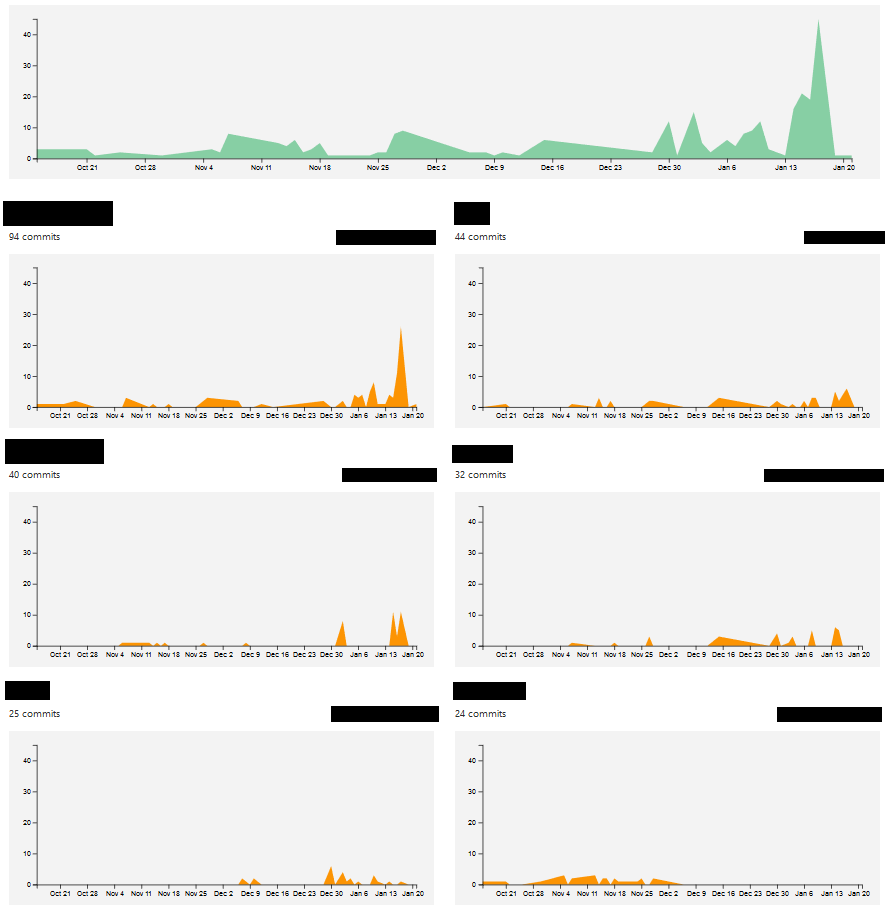
\includegraphics[scale=0.4]{slike/aktivnost.PNG} %veličina slike u odnosu na originalnu datoteku i pozicija slike
			\centering
			\caption{Primjer slike s potpisom}
			\label{fig:promjene}
		\end{figure}
		
		\begin{figure}[H]
			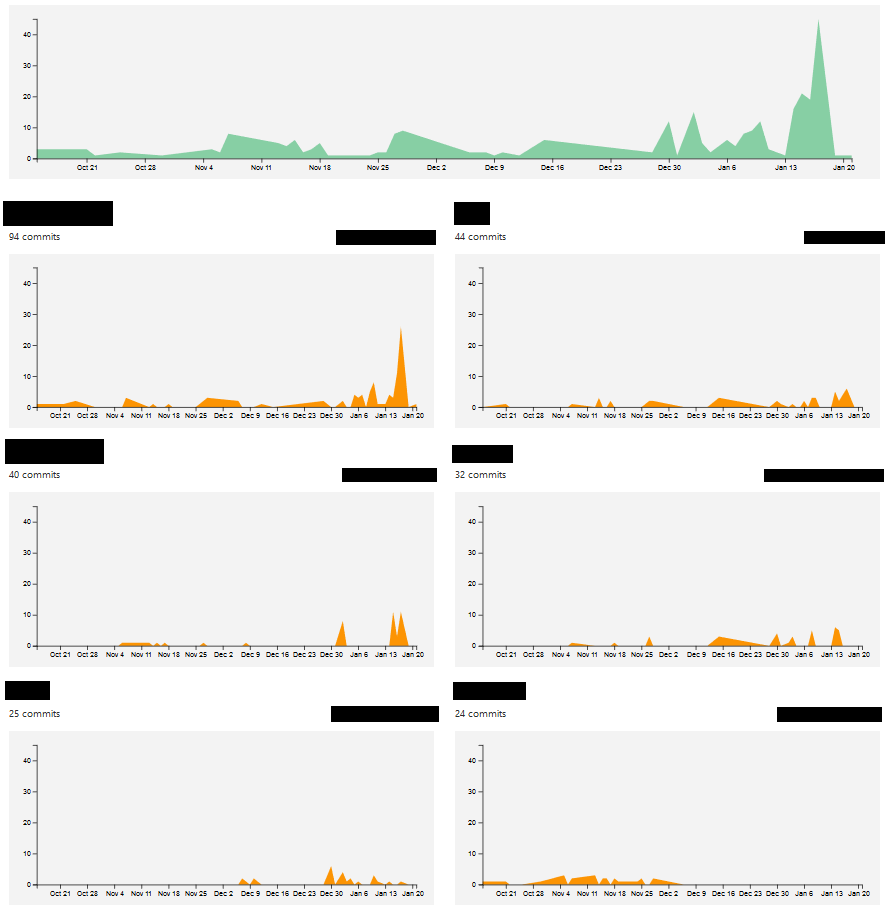
\includegraphics[width=\textwidth]{slike/aktivnost.PNG} %veličina u odnosu na širinu linije
			\caption{Primjer slike s potpisom 2}
			\label{fig:promjene2} %label mora biti drugaciji za svaku sliku
		\end{figure}
		
		Referenciranje slike \ref{fig:promjene2} u tekstu.
		
		\eject
		
	